\documentclass{article}
\usepackage[utf8]{inputenc}
\usepackage{graphicx}
\usepackage{amsmath}
\usepackage{hyperref}

\graphicspath{ {./data/} }

\title{E17e Coupled Electrical Oscillations Report}
\author{Adam Kit}
\date{May 2020}


\begin{document}

\maketitle
\begin{equation}
\end{equation}
\section*{Preperation}
In this experiment two \textit{LC} resonant circuits are coupled either by a capacitance or by a mutual inductance. The capacitor in one of the circuits is charged by applying a DC voltage. This circuit is excited to oscillations by the subsequent removal of the voltage and the coupled oscillations of both circuits aremeasured as a function of time. From this the resonant frequencies are determined and their dependence on coupling capacitance or mutual inductance is studied.

To set this up, Prof. Ziesse provided us with data recorded using a PC Oscilloscope.
\subsection{Fourier  Coefficients}
To approximate a function with a Fourier series we need a periodic bounded function that is integrable over a period $T$. If that is achieved, then we can write the function as the following series:
\begin{equation}
f(x) = a_0 + \sum_{n=1}^{\infty}[a_n cos(\omega_n t)+ b_nsin(\omega_n t)]
\end{equation}


where frequency $\omega_n$ is defined by $\omega_n = \frac{2 \pi n}{T}$. The coefficients are then found with the following equations
\begin{equation}
a_0 = \int_0^T f(t)dt
\end{equation}
\begin{equation}
a_n = \frac{2}{T}\int_{-\frac{T}{2}}^{\frac{T}{2}} f(t)cos(\omega_nt)dt
  \quad\text{and}\quad
b_n = \frac{2}{T}\int_{-\frac{T}{2}}^{\frac{T}{2}} f(t)sin(\omega_nt)dt
\end{equation}

For the square wave represented in the Figure
\begin{figure}[h]
  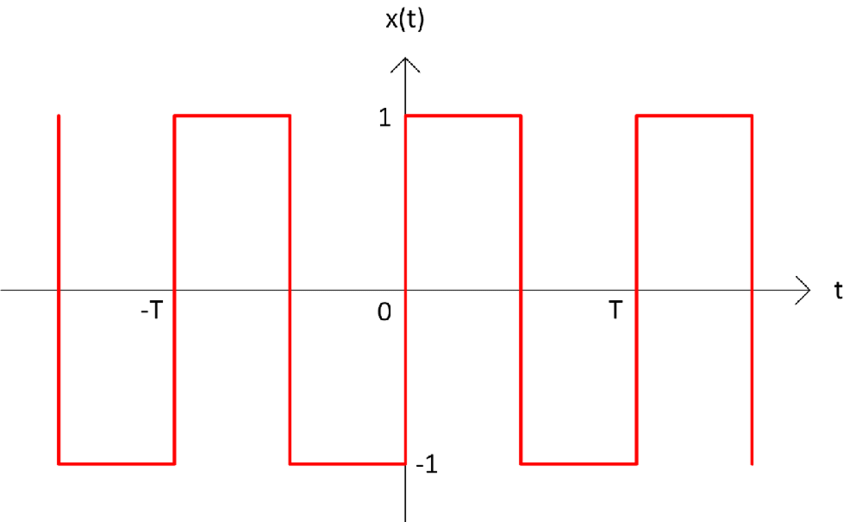
\includegraphics[scale=0.5]{squarewave.png}
  \caption{Here the light in the far field (blue line and variables) is simple the fourier transform of the apertured field (red line and variables)}
\end{figure}

We find the fourier coefficients by using the equaitons 1, 2, 3.

Triangle:

\subsection{FFT}
sine, triangle, square
\subsection{Comparison}
Triangle -> Triangle FFT
SQUARE -> Square FFT

\section{Aliasing}
Explain what the alias effect is. Why do these measurements prove the alias effect? If a measurement is made of a sine voltage with a frequency of 44.5 kHz with oscilloscope settings as shown to the right, how does the spectrum look like?



\section{Square Voltage}
Why do the spectra look so different? Compare qualitatively to your calculations from task 0.

\section{Triangular Voltage}
Why do the spectra look so different? Compare qualitatively to your calculations from task 0.Why does the lower time trace consist of a triangular pattern?
\section{Low-Point Circuit}
Draw the wiring for the low-point circuit into the image and include the result in your lab report.

\section{High-Point Circuit}
Draw the wiring for the high-point circuit into the image and include the result in your lab report.

\begin{thebibliography}{9}
\bibitem{latexcompanion}
James W. Cooley and John W. Tukey
\textit{An algorithm for the machine calculation of complex Fourier series}.
Math. Comp. 19 (1965)

\bibitem{optics}
Brooker, Geoffrey
\textit{Modern Classical Optics}
Oxford: Oxford University Press (2003)
\end{thebibliography}










\end{document}
